\section{Zero signed-weight residues: the eight-cycle geometry}\label{sec:zero-d-cycle}
Normalize the source so that $d+\sum_i c_i=1$. Suppose $\bar d=0$ and both testing measurement pairs are noncommuting in residue. A projective choice of testing frame gives finite residue half angles with $u_0v_0\ne0$. The following classification uses only the geometry of product vectors.

\begin{lemma}[Product residues are already settled]
At noncommuting residue angles every product state satisfies $H>0$. Consequently the entire parent is tensor SOS whenever its residue state is product.
\end{lemma}
\begin{proof}
For a product state,
\[
S=a_0(b_0-b_1)+a_1(b_0+b_1)
\le |b_0-b_1|+|b_0+b_1|=2\max(|b_0|,|b_1|)\le2.
\]
If both Bob moduli are less than one, the inequality is strict. Otherwise precisely one is one, since noncommuting qubit reflections have no common eigenvector. Both $b_0-b_1$ and $b_0+b_1$ are then nonzero; equality would require $|a_0|=|a_1|=1$, again impossible. Thus $H=1-S/2>0$ at the residue. Its actual testing value remains positive. The signed term $d\otimes(D_uD_vH)$ is therefore a square after separate field square roots, and every event term is already a positive weighted square.
\end{proof}

The losing events form a single bipartite cycle between the four Alice and four Bob outcome rays:
\begin{center}
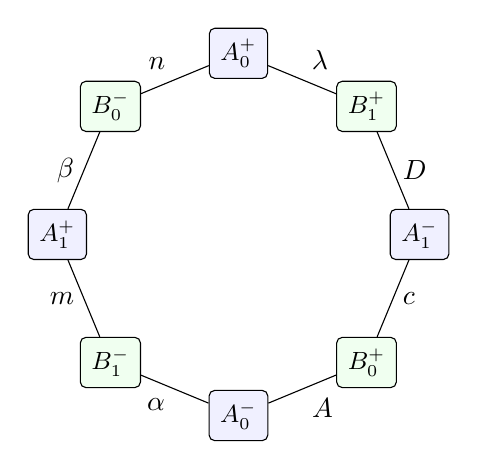
\begin{tikzpicture}[vertex/.style={draw,rounded corners=2pt,inner sep=4pt,font=\small},every edge/.style={draw,thick}]
\node[vertex,fill=blue!6] (a0) at (90:23mm) {$A_0^+$};
\node[vertex,fill=green!6] (b1) at (45:23mm) {$B_1^+$};
\node[vertex,fill=blue!6] (a1) at (0:23mm) {$A_1^-$};
\node[vertex,fill=green!6] (b0) at (-45:23mm) {$B_0^+$};
\node[vertex,fill=blue!6] (a2) at (-90:23mm) {$A_0^-$};
\node[vertex,fill=green!6] (b2) at (-135:23mm) {$B_1^-$};
\node[vertex,fill=blue!6] (a3) at (180:23mm) {$A_1^+$};
\node[vertex,fill=green!6] (b3) at (135:23mm) {$B_0^-$};
\draw (a0)--node[above right] {$\lambda$}(b1);
\draw (b1)--node[right] {$D$}(a1);
\draw (a1)--node[right] {$c$}(b0);
\draw (b0)--node[below right] {$A$}(a2);
\draw (a2)--node[below left] {$\alpha$}(b2);
\draw (b2)--node[left] {$m$}(a3);
\draw (a3)--node[left] {$\beta$}(b3);
\draw (b3)--node[above left] {$n$}(a0);
\end{tikzpicture}
\end{center}
For example, $\lambda,D$ share Bob's ray $B_1^+$, while $D,c$ share Alice's ray $A_1^-$. The eight local rays are distinct within their respective parties at noncommuting angles.

\begin{theorem}[Exhaustive noncommuting zero-$d$ residue classification]
An unresolved zero residue has an entangled state. Its positive-residue event support is a matching in the eight-cycle, hence has at most four elements.

For a support of size $k\le3$, the event residue has Hessian rank $k$ in the five angle-and-projective-state variables. Its zero locus is smooth of dimension $5-k$. For four events the only possibilities are
\[
\{n,m,A,D\},\quad u_0^2=v_0^2;
\qquad
\{\lambda,c,\alpha,\beta\},\quad u_0^2v_0^2=1.
\]
Each has state rank three and one additional angular normal, so its full Hessian rank is four and its zero locus has dimension one. There are no further exceptional noncommuting loci.
\end{theorem}
\begin{proof}
At $\bar d=0$, vanishing of the nonnegative event sum forces every positive-weight event amplitude to vanish. Write the real state as a $2\times2$ matrix $\Psi$. Entanglement means $\det\Psi\ne0$. For each fixed nonzero Alice ray $a$, the equation $a^T\Psi b=0$ determines a unique Bob projective ray, and conversely. Vanishing events therefore share no vertex: they form a matching.

Any three distinct product vectors in this event system are linearly independent. Indeed, three dependent rank-one matrices must share a left factor or share a right factor. If the first two have both independent left and independent right factors, their span is diagonal in suitable bases and contains only those two rank-one projective points. If they share a factor, their entire span shares it. A cycle vertex has degree two, so three event vectors cannot share a factor. For $k\le3$, the $k$ independent state-linear amplitudes have derivative rank $k$ on the projective state chart at their common zero. The implicit-function theorem and the formula for the Hessian of a sum of squared vanishing functions give the stated rank and smooth zero set.

An even cycle has exactly two perfect matchings. For $\{n,m,A,D\}$ the equations give $X=Y=0$, $vW-uZ=uW-vZ=0$. A nonzero solution exists precisely on $u^2=v^2$. Put $W=1$, $v=\sigma u$, $Z=\sigma$ with $\sigma=\pm1$. After removing the independent $X,Y$ normals, the other two derivatives in $(u,v,Z)$ are
\[
(-\sigma,1,-u),\qquad(1,-\sigma,-\sigma u).
\]
They are independent because $u\ne0$. Thus the full rank is four.

For $\{\lambda,c,\alpha,\beta\}$, put $W=1$. The first three equations give $X=-1/v$, $Y=u$, $Z=uv$. The fourth becomes $(u^2v^2-1)/v=0$, with nonzero angular gradient. Again there are three state normals and one angular normal. These descriptions also show directly that the signed core vanishes on the two curves.
\end{proof}

\begin{corollary}[Adjacent dominant events need no noncommuting atlas]
If two positive-residue event coefficients share an outcome ray, the entire parent is tensor SOS at every noncommuting residue test.
\end{corollary}
\begin{proof}
Positive slack residue is already settled by Lemma~\ref{lem:residue}. At a zero residue, the two amplitudes sharing a ray force a product kernel state: two distinct rays at the other party span its two-dimensional space. The preceding product-state lemma applies.
\end{proof}

The two canonical families reduce the matching list further. For $C_1$ the only three-event matchings are $\{m,A,D\}$, $\{c,\alpha,\beta\}$, $\{A,D,\beta\}$ and $\{D,\alpha,\beta\}$; there is no four-event matching. For $C_2$ they are $\{n,m,c\}$, $\{n,m,A\}$, $\{n,m,D\}$, $\{n,c,\alpha\}$, $\{n,A,D\}$, $\{n,D,\alpha\}$ and $\{m,A,D\}$; only $\{n,m,A,D\}$ can have four events.

\paragraph{A two-variable scalar restriction.}
The nonextendable matching $\{\lambda,m,A\}$ has polynomial kernel state
\[
(W,X,Y,Z)=(uv,-u,0,1+v^2).
\]
Substitute this state into the entire parent and divide by the positive pure testing factor $2u^2v^2(1+v^2)$. With $U=u^2,V=v^2$, the result is exactly
\[
L(U,V)=\frac{2n(1+U)}V+2cU+\frac{2D(1+V)}U
 +\frac{2\alpha(1+U)(1+V)}{UV}+2\beta V-d.
\]
Physicality implies $L\ge0$ on the positive quadrant. In particular,
$d\le4n+2c+4D+8\alpha+2\beta$. Thus at least one complementary event weight is not infinitesimal relative to $d$. The other seven nonextendable triples give analogous exact restrictions by their polynomial kernel states.

\status{The cycle gives the support geometry, not by itself the full-parent certificate. The following weighted normal completions retain every normal cross term and handle one, two, three and four hard event constraints at arbitrary coefficient scales. The finite induction in Theorem~\ref{thm:all-noncommuting} completes every noncommuting residue test. It does not assume that an extreme source has three positive-residue event weights.}
